\section{Runtime scheduler}
Come vengono messi in attesa o svegliate le goroutine? \newline Questo viene gestito dal runtime scheduler, il suo lavoro e' quello di distribuire le goroutine (G) sui diversi OS thread (M) che vengono eseguiti su uno o piu processori (P).

\begin{figure}[h!]
    \centering
    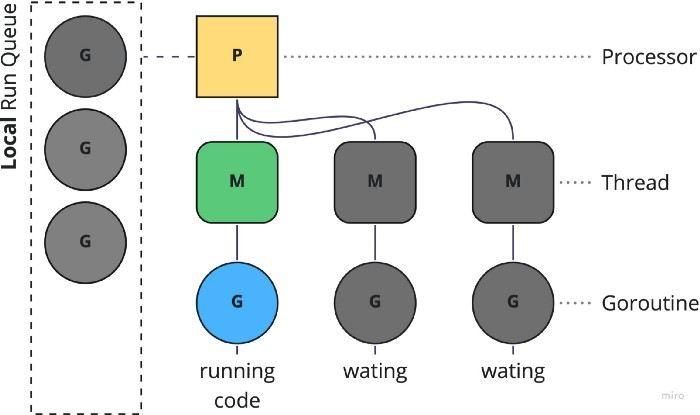
\includegraphics[width=10cm]{sections/runtime-go2.jpeg}
    \caption{go runtime scheduler}
    \label{fig:title}
\end{figure}

Dall'immagine abbiamo 3 oggetti diversi:

\begin{itemize}
    \item P: Processore
    \item M: OS/Kernel thread
    \item G: goroutine
\end{itemize}

Il numero di P e' stabilito dalla variabile di ambiente \textbf{GOMAXPROCS}, in generale e' pari al numero di core presenti sul nostro processore. \newline
Quando una goroutine viene creata, o quando il suo stato divena runnable, viene inserita all'interno di una lista di goroutine runnable, (P) cerchera di prendere la prima goroutine dalla lista, se la lista e' vuota ruba agli altri (P) meta delle loro goroutine. \newline
Go gestisce due liste, la lista globale e la lista locale ad ogni processore. Una goroutine finisce sulla lista globale solo se tutte quelle locali sono piene.

\begin{figure}[h!]
    \centering
    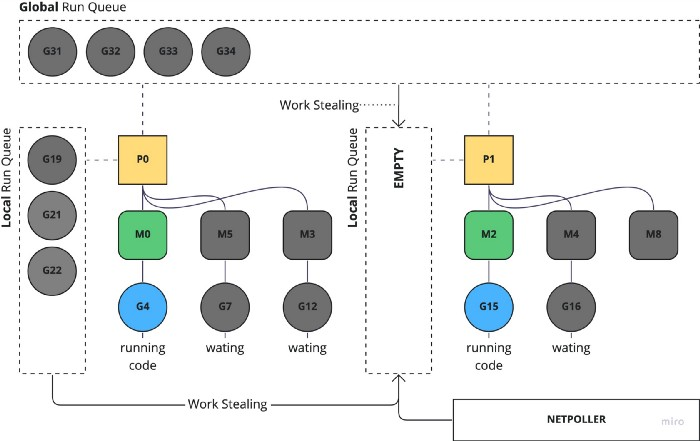
\includegraphics[width=12cm]{sections/runtime-go3.jpeg}
    \caption{go runtime scheduler}
    \label{fig:title}
\end{figure}

Dall'immagine sopra vediamo che P1 non ha piu goroutine, quindi il Go runtime scheduler prendera le goroutine dagli altri processori. Se ogni processore non ha goroutine controllera se ci sono delle operazioni di IO, per esempio syscall o network request, da eseguire dal netpoller. Se il netpoller e' vuoto il processore cerchera di prendere le goroutine dalla lista globale.